% begin module concavity-def
\begin{frame}
\frametitle{What Does $f''$ Say About $f$?}
$f$ and $g$ are both increasing on $(a,b)$, but ``bend'' in different directions.
\begin{columns}[c]
\column{.5\textwidth}
\psset{xunit=0.6cm, yunit=0.6cm}
\begin{pspicture}(-1,-1)(4,3.8)
\psframe*[linecolor=white](-1,-1)(4,3.8)
\psaxes[ticks=none, labels=none]{<->}(0,0)(-1,-1)(4,3.8)
%Function formula: 1/2+1/4 ((-1+x)^{2})+1/4 (x) =1/4x^{2}-1/4x +3/4
\psplot[linecolor=red, plotpoints=1000]{-1}{4}{x 0.25 mul x -1 add 2 exp 0.25 mul add 0.5 add }
\tiny
\rput(1, 2){$y=f(x)$}
\psXTickWithLabel{0.5}{$a$} 
\psXTickWithLabel{3.7}{$b$} 

\uncover<3>{ %point: x=0.3
%Function formula: -1/10 (x)+291/400 
\psplot[linecolor=blue, plotpoints=1000]{-0.5}{4}{0.7275 x -0.1 mul add }
}
\uncover<4->{%point: x=0.3
%Function formula: -1/10 (x)+291/400 
\psplot[linecolor=blue, plotpoints=1000]{0}{0.6}{0.7275 x -0.1 mul add } 
}
\uncover<3->{
\psFullDot{0.3}{0.6975}
}

\uncover<4>{ %point x=1.3
%Function formula: 2/5 (x)+131/400 
\psplot[linecolor=blue, plotpoints=1000]{-0.5}{4}{0.3275 x 0.4 mul add } 
}
\uncover<5->{ %point x=1.3
%Function formula: 2/5 (x)+131/400 
\psplot[linecolor=blue, plotpoints=1000]{1}{1.6}{0.3275 x 0.4 mul add } 
}
\uncover<4->{
\psFullDot{1.3}{0.8475}
}

\uncover<5>{ %point x=2.3
%Function formula: 9/10 (x)-229/400 
\psplot[linecolor=blue, plotpoints=1000]{0.080555556}{4}{-0.5725 x 0.9 mul add } 
}
\uncover<6->{ %point x=2.3
%Function formula: 9/10 (x)-229/400 
\psplot[linecolor=blue, plotpoints=1000]{2}{2.6}{-0.5725 x 0.9 mul add } 
}
\uncover<5->{
\psFullDot{2.3}{1.4975}
}

\uncover<6>{ %point x=3.3
%Function formula: 7/5 (x)-789/400 
\psplot[linecolor=blue, plotpoints=1000]{1.051785714}{4}{-1.9725 x 1.4 mul add } 
}
\uncover<7->{  %point x=3.3
%Function formula: 7/5 (x)-789/400 
\psplot[linecolor=blue, plotpoints=1000]{3}{3.6}{-1.9725 x 1.4 mul add } 
}
\uncover<6->{
\psFullDot{3.3}{2.6475}
}
\uncover<9>{
\psline[linecolor=blue](-1, 1.25) (1.6, 0.99)
}
\uncover<10->{
\psline[linecolor=blue!30](-1, 1.25) (1.6, 0.99)
}
\uncover<10>{
\psline[linecolor=blue](0, 0.75) (2.6, 1.79)
}
\uncover<11->{
\psline[linecolor=blue!30](0, 0.75) (2.6, 1.79)
}
\uncover<11>{
\psline[linecolor=blue](1, 0.75) (3.6, 3.09)
}
\uncover<12->{
\psline[linecolor=blue!30](1, 0.75) (3.6, 3.09)
}

\rput[t](2,-0.5) {\uncover<6->{Concave up}}
\end{pspicture} 
%\ \only<handout:0| -2>{%
%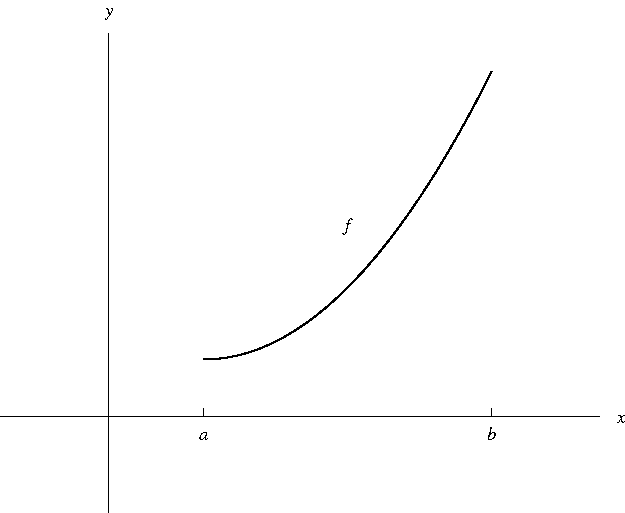
\includegraphics[height=3.5cm]{curve-sketching/pictures/04-03-concaveupa.pdf}%
%}%
%\only<handout:0| 3>{%
%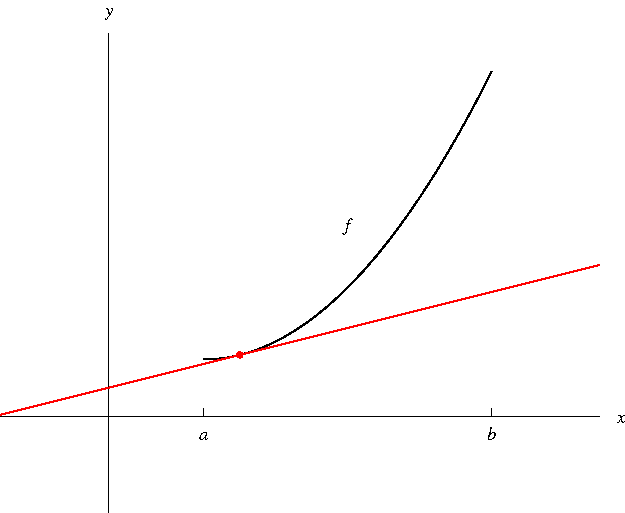
\includegraphics[height=3.5cm]{curve-sketching/pictures/04-03-concaveupb.pdf}%
%}%
%\only<handout:0| 4>{%
%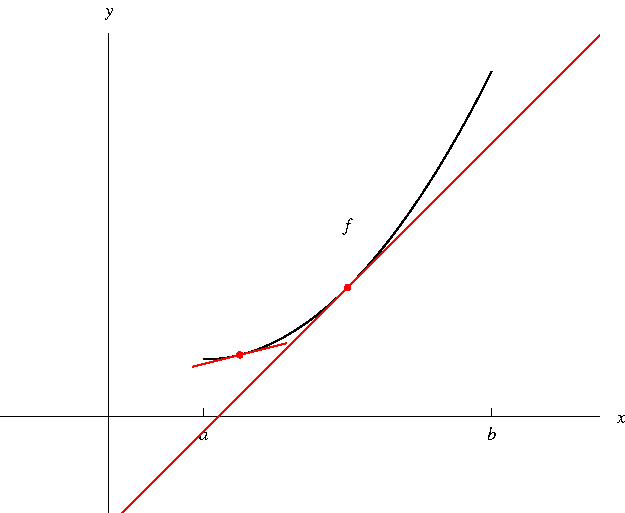
\includegraphics[height=3.5cm]{curve-sketching/pictures/04-03-concaveupc.pdf}%
%}%
%\only<handout:0| 5>{%
%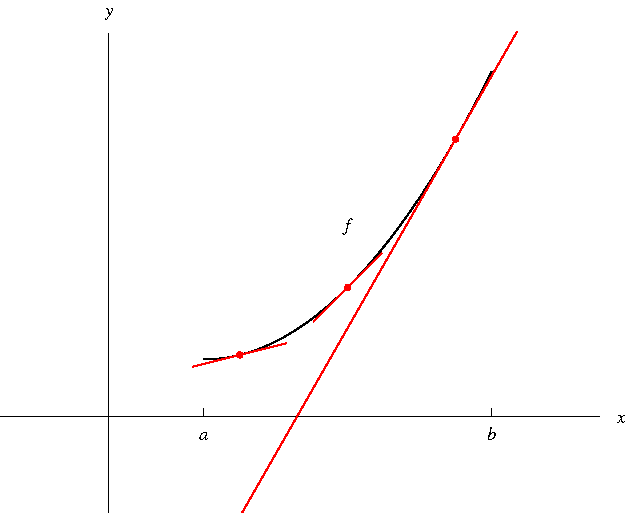
\includegraphics[height=3.5cm]{curve-sketching/pictures/04-03-concaveupd.pdf}%
%}%
%\only<6->{%
%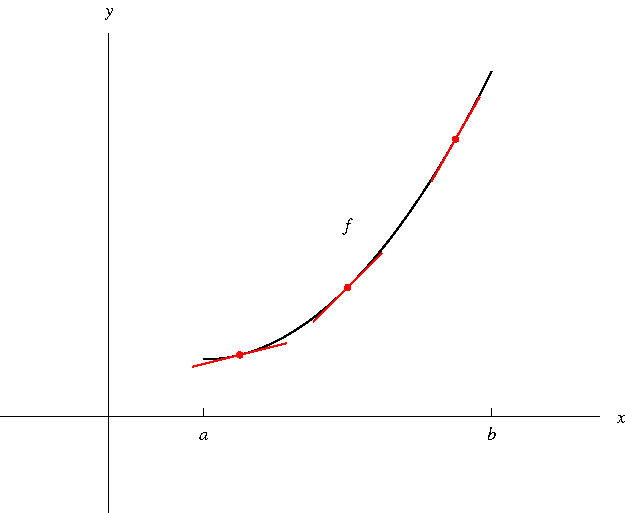
\includegraphics[height=3.5cm]{curve-sketching/pictures/04-03-concaveupe.pdf}%
%}%


\column{.5\textwidth}
\psset{xunit=0.6cm, yunit=0.6cm}
\begin{pspicture}(-1,-1)(4,3.8)
\psframe*[linecolor=white](-1,-1)(4,3.8)
\psaxes[ticks=none, labels=none]{<->}(0,0)(-1,-1)(4,3.8)
\tiny
\rput[l](2.5, 0.7){$y=g(x)$}
%Function formula: -1/4x^{2}+5/4x +1/2=11/4-1/4 (-3+x)^{2}-1/4 x 
\psplot[linecolor=red, plotpoints=1000]{-1}{4}{x -0.25 mul x -3 add 2 exp -0.25 mul add 2.75 add }
\psXTickWithLabel{0.3}{$a$} 
\psXTickWithLabel{2.5}{$b$} 


\uncover<3>{
%Function formula: 11/10 (x)+209/400 
\psplot[linecolor=blue, plotpoints=1000]{-0.5}{2.979}{0.5225 x 1.1 mul add }
}
\uncover<4->{ 
%Function formula: 11/10 (x)+209/400 
\psplot[linecolor=blue, plotpoints=1000]{0}{0.6}{0.5225 x 1.1 mul add } 
}
\uncover<3->{
\psFullDot{0.3}{0.8525}
}
\uncover<4>{
%Function formula: 3/5 (x)+369/400 
\psplot[linecolor=blue, plotpoints=1000]{-0.5}{4}{0.9225 x 0.6 mul add } 
}
\uncover<5->{
%Function formula: 3/5 (x)+369/400 
\psplot[linecolor=blue, plotpoints=1000]{1}{1.6}{0.9225 x 0.6 mul add } 
}
\uncover<4->{
\psFullDot{1.3}{1.7025}
}

\uncover<5>{
%Function formula: 1/10 (x)+729/400 
\psplot[linecolor=blue, plotpoints=1000]{-0.5}{4}{1.8225 x 0.1 mul add } 
}
\uncover<6->{
%Function formula: 1/10 (x)+729/400 
\psplot[linecolor=blue, plotpoints=1000]{2}{2.6}{1.8225 x 0.1 mul add } 
}
\uncover<5->{
\psFullDot{2.3}{2.0525}
}
\uncover<6>{
%Function formula: -2/5 (x)+1289/400 
\psplot[linecolor=blue, plotpoints=1000]{-0.5}{4}{3.2225 x -0.4 mul add } 
}
\uncover<7->{
%Function formula: -2/5 (x)+1289/400 
\psplot[linecolor=blue, plotpoints=1000]{3}{3.6}{3.2225 x -0.4 mul add } 
}
\uncover<6->{
\psFullDot{3.3}{1.9025}
}
\rput[t](2,-0.5) {\uncover<6->{Concave down}}
\uncover<9>{
\psline[linecolor=blue] (-1, -1) (1.6, 1.86)
}
\uncover<10->{
\psline[linecolor=blue!30] (-1, -1) (1.6, 1.86)
}
\uncover<10>{
\psline[linecolor=blue] (0, 0.5) (2.6, 2.06)
}
\uncover<11->{
\psline[linecolor=blue!30] (0, 0.5) (2.6, 2.06)
}
\uncover<11>{
\psline[linecolor=blue] (1, 1.5) (3.6, 1.76)
}
\uncover<12->{
\psline[linecolor=blue!30] (1, 1.5) (3.6, 1.76)
}

\end{pspicture} 
%\ \only<handout:0| -2>{%
%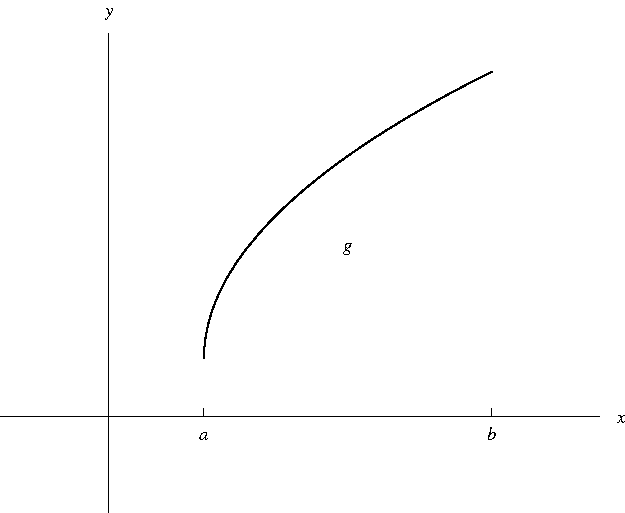
\includegraphics[height=3.5cm]{curve-sketching/pictures/04-03-concavedowna.pdf}%
%}%
%\only<handout:0| 3>{%
%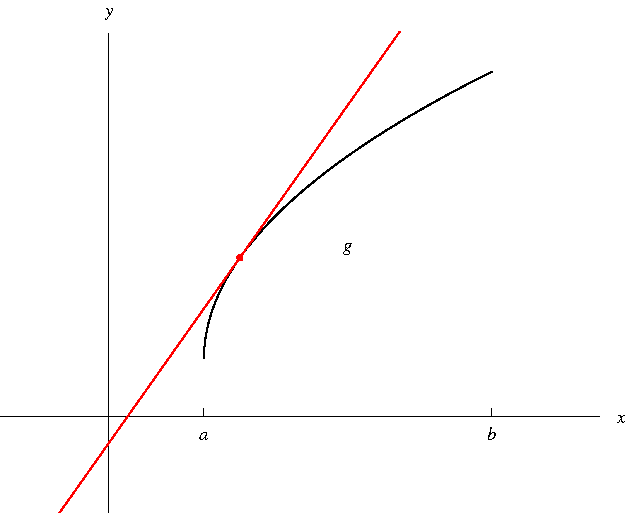
\includegraphics[height=3.5cm]{curve-sketching/pictures/04-03-concavedownb.pdf}%
%}%
%\only<handout:0| 4>{%
%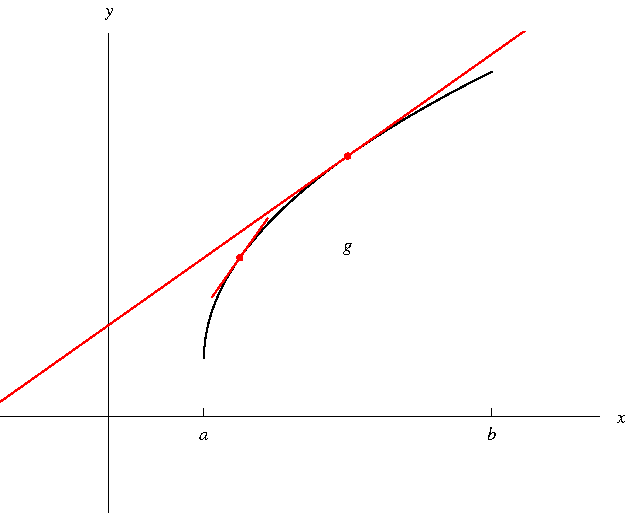
\includegraphics[height=3.5cm]{curve-sketching/pictures/04-03-concavedownc.pdf}%
%}%
%\only<handout:0| 5>{%
%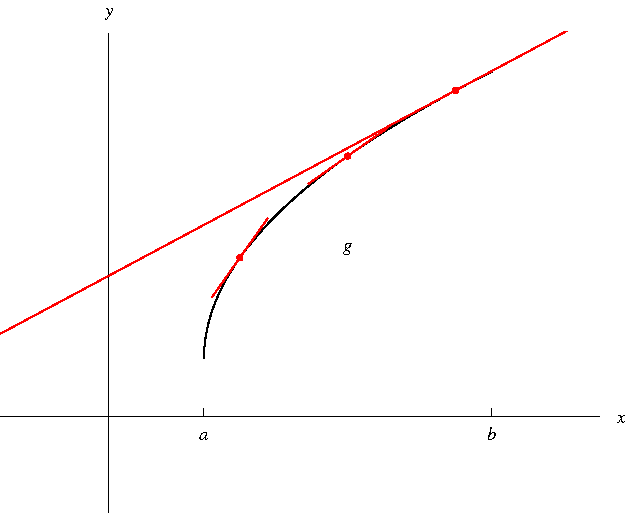
\includegraphics[height=3.5cm]{curve-sketching/pictures/04-03-concavedownd.pdf}%
%}%
%\only<6->{%
%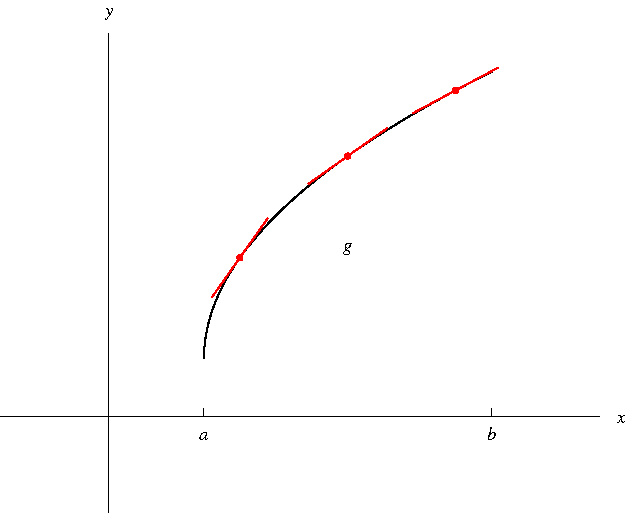
\includegraphics[height=3.5cm]{curve-sketching/pictures/04-03-concavedowne.pdf}%
%}%
\end{columns}
\uncover<8-12>{%
\begin{definition}[Concave Up/Concave Down, most general definition]
A function is called concave up/down if the line segment between any two points on its graph lies above/below the graph.
\end{definition}
}%
\uncover<2->{
\begin{theorem}[Can be taken as a definition]
Let $f$ be a differentiable function on an interval $I$. Then $f$ is
concave up (on $I$) if its graph lies above all of its tangents (on $I$), and $f$ is concave down (on $I$) if its graph lies below all of its tangents (on $I$).
\end{theorem}
}
\end{frame}
% end module concavity-def
